% This file should be rename with the speaker's last name. (e.g : smith)

% Write the author names in the order you wish them to appear
% and underline the one who will give the talk.

% Only the speaker's email address is required.

\begin{abstract_online}{GeoGebra Automated Reasoning Tools: \\ a problem from Spanish Civil Service \\ Math Teachers' examination}{%
        \underline{M.Pilar V\'elez}$^{1}$, Zolt\'an Kov\'acs,$^{2}$, Tom\'as Recio $^{3}$}{[pvelez@nebrija.es]
        }{%
        $^1$ Universidad Antonio de Nebrija,  Madrid, Spain \newline{}$^2$ The Private University College of Education of the Diocese of Linz,  Austria \newline{}$^3$ Universidad de Cantabria,  Santander, Spain}
    
GeoGebra is open source software, freely available for non-commercial users. It is dynamic mathematics software that brings together geometry, algebra, spreadsheets, graphing, statistics and calculus in one easy-to-use package,  for all levels of education.


 In 2013, Bernard Parisse's software
 Giac\footnote{\url{https://www-fourier.ujf-grenoble.fr/~parisse/giac.htm}}
 was integrated into GeoGebra's Computer Algebra System view. This
 allowed to include some automated reasoning tools (ART) in GeoGebra, for
 mechanically finding relations among geometric elements, for testing the
 truth or falsity of some statement, for finding additional hypotheses
 for a given statement to hold, cf.~[1], [2]. The algorithms behind these
 tools are  based in computational algebraic geometry, cf.~[3].



On the other hand, the Spanish recruitment method to become a civil servant math teacher for the  secondary school system  requires passing and getting the best grades on  a series of  exams (``oposiciones''). In one of these recent tests, the candidates were requested to solve an elementary geometry question, asking to conjecture,  formulate and,  then,  to prove,  the ratio holding between  two  particular segments in a given figure (see Fig. \ref{fig1}).



\begin{figure}[h]
 \centering

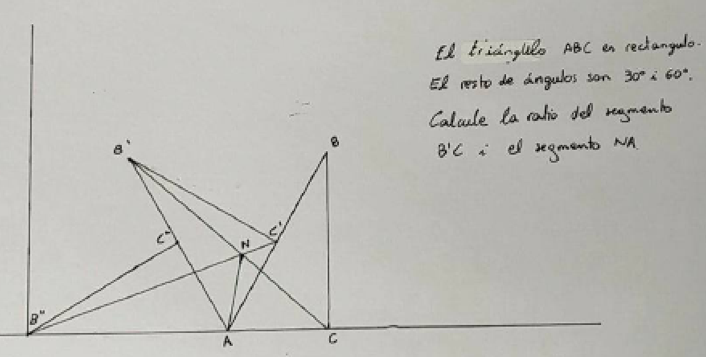
\includegraphics[scale=0.7]{example1}\caption{Geometric question from a
recent Spanish Math Teachers' recruitment examination: \emph{Triangle $ABC$
is right-angled. The rest of the angles are $30^{\textrm o}$ and $60^{\textrm o}$. Find the
ratio between segment $B'C$ and $NA$}} 

\label{fig1}   
\end{figure}



We used GeoGebra ART to accomplish this task, showing, on the one hand,
how much it simplifies solving the posed problem; and, on the other, the
relevance to adapt and simplify our algorithmic formulation based in
elimination ideals [3], to the special zero-dimensional case.

 In fact, this example shows that  some quite natural,  human
 interpretations of the given situation could lead to a complicated
 ``truth on parts'' conclusion (cf.~[4]), in which the thesis will
 simultaneously hold and fail over some irreducible components of the
 algebraic variety describing the set of instances verifying the
 hypotheses.
 
 This will imply, in particular,  the need to optimize, for the zero dimensional case, the formulation of the algorithms for detecting ``truth on parts'', thus warning the user about some  hidden, unexpected problem that requires further analysis from his/her side.

Our talk with address both the issues related to the mathematical improvements of the automated reasoning algorithms that this example has suggested,  as well as the analysis of the desirable interrelation human/machine that could be behind a future scenario towards improving the chances of ``passing'' the ``oposiciones''  examination.

\textbf{Keywords} \newline{} Dynamic Geometry, Automated Reasoning, GeoGebra

\textbf{References} \newline{}
[1] \textsc{M.A. Ab\'anades, F. Botana, Z. Kov\'acs, T. Recio, C. S\'olyom-Gecse}, Development of automatic reasoning tools in GeoGebra. \emph{ACM Communications in Computer Algebra} \textbf{50}(30), 85--88  (2016). \newline{}
 [2] \textsc{Z. Kov\'acs, T. Recio, M. P. V\'elez}, Using Automated Reasoning Tools in GeoGebra in the Teaching and Learning of Proving in Geometry. \emph{International Journal of Technology in Mathematics Education} \textbf{25}(2), 33--50  (2018). \newline{}
 [3] \textsc{T. Recio, M. P. V\'elez}, Automatic discovery of theorems in elementary geometry. \emph{Revista Matem\'atica Complutense} \textbf{23}, 63--82 (1999). \newline{}
 [4] \textsc{Z. Kov\'acs, T. Recio, M. P. V\'elez}, Detecting truth, just on parts. \emph{Revista Matem\'atica Complutense},
\url{https://doi.org/10.1007/s13163-018-0286-1} (2018). \newline{}
\end{abstract_online}
    